\documentclass[11pt]{article}
\usepackage[margin=1in]{geometry}
\usepackage{graphicx}
\usepackage{booktabs}
\usepackage{tabularx}
\usepackage{hyperref}
\usepackage{url}
\usepackage{enumitem}
\setlist{nosep}
\usepackage[skip=4pt]{caption}
\usepackage{float}
\setlength{\emergencystretch}{1em}
\makeatletter\g@addto@macro\UrlBreaks{\do\_\do\=}\makeatother % long identifiers may break after _ and =

% All acceptance numbers come from report/make_results_tex.py (re-run it after a new acceptance run).
% Generated by report/make_results_tex.py -- do not edit by hand.
\newcommand{\AcceptanceRows}{%
\multicolumn{6}{l}{\textbf{Run 1}: \texttt{warehouse\_models\_person}, detector \texttt{7241462}, threads default; 2/3 reached} \\
\quad\texttt{go to person 0} & \texttt{person\_0} & -- & -- & -- & skipped$^{*}$ \\
\quad\texttt{go to person 1} & \texttt{person\_1} & 0.08 & 0.85 & 13.2 & reached \\
\quad\texttt{go to person 2} & \texttt{person\_2} & 0.03 & 0.71 & 18.0 & reached \\
\midrule
\multicolumn{6}{l}{\textbf{Run 2}: \texttt{warehouse\_models}, detector \texttt{6e7f4db}, threads default; 2/3 reached} \\
\quad\texttt{go to person 0} & \texttt{person\_0} & 0.07 & 0.78 & 16.6 & reached \\
\quad\texttt{go to trash can} & \texttt{trash\_can\_0} & 0.04 & 0.81 & 11.0 & reached \\
\quad\texttt{go to chair} & \texttt{chair\_0} & 0.27 & 2.74 & 60.3 & failed \\
\midrule
\multicolumn{6}{l}{\textbf{Run 3}: \texttt{warehouse\_models\_person}, detector \texttt{ddf8335}, threads 4; 2/3 reached} \\
\quad\texttt{go to person 0} & \texttt{person\_0} & 0.23 & 0.82 & 7.2 & reached \\
\quad\texttt{go to person 1} & \texttt{person\_1} & -- & -- & -- & skipped$^{*}$ \\
\quad\texttt{go to person 2} & \texttt{person\_2} & 0.02 & 0.78 & 19.2 & reached \\
}
\newcommand{\NRuns}{3}
\newcommand{\NCmds}{9}
\newcommand{\NNavigable}{7}
\newcommand{\NReached}{6}
\newcommand{\NLandmarks}{7}
\newcommand{\LmErrMin}{0.02}
\newcommand{\LmErrMax}{0.27}
\newcommand{\DistMin}{0.71}
\newcommand{\DistMax}{0.85}


\newcommand{\repo}{https://github.com/DylanDai63/cse498-lab3a}

\title{CSE 398/498 Lab 3a Report:\\How a Language Command Drives a Simulated TurtleBot3 to an Object}
\author{Hengde Dai \\ \texttt{hed424@lehigh.edu}}
\date{October 4, 2026}

\begin{document}

\maketitle

\begin{center}
\fbox{\parbox{0.92\textwidth}{\centering
\textbf{GitHub repository (code, demo video, acceptance results, report source):}\\[2pt]
\large\url{\repo}\\[2pt]
\normalsize Demo video (two commands): \path{videos/lab3a_demo.mp4} in the repository
}}
\end{center}

\section{Overview}

The lab workspace is a ROS~2 Humble system in which a simulated TurtleBot3 Waffle Pi explores an unknown room in Gazebo, builds a SLAM map, recognizes three kinds of objects (person, trash can and chair) and remembers where they are on the map. A user then names an object in a short text command, and the robot drives to it. The design is ``map first, query later'': a command is a lookup in the semantic map that the robot built while exploring, not a search for the object (Figure~\ref{fig:overview}).

Gazebo itself only simulates the robot and the room. It publishes the camera images, the laser scan and the wheel odometry, and it moves the robot according to the velocity commands on \texttt{/cmd\_vel}. Everything that ``digests'' a command, namely parsing, perception, mapping and planning, runs in ROS~2 nodes outside the simulator.

Everything except the object detector is provided by the course repository. The coding part of this lab was to implement \texttt{load()} and \texttt{infer()} in \path{src/tb3_detector/tb3_detector/detector_core.py}, and this is the only source file I changed. I ran the workspace on my laptop in WSL~2 (Ubuntu 22.04, ROS~2 Humble, Gazebo Classic 11), which is the Windows setup documented in the repository.

Sections~\ref{sec:command} to~\ref{sec:nav} follow one command through the system in the order the assignment asks for: how the command is given and parsed, how camera images become object positions, how the SLAM map is used, and how the robot drives to the goal. Section~\ref{sec:results} reports the acceptance runs and the demo video.

\begin{figure}[H]
\centering
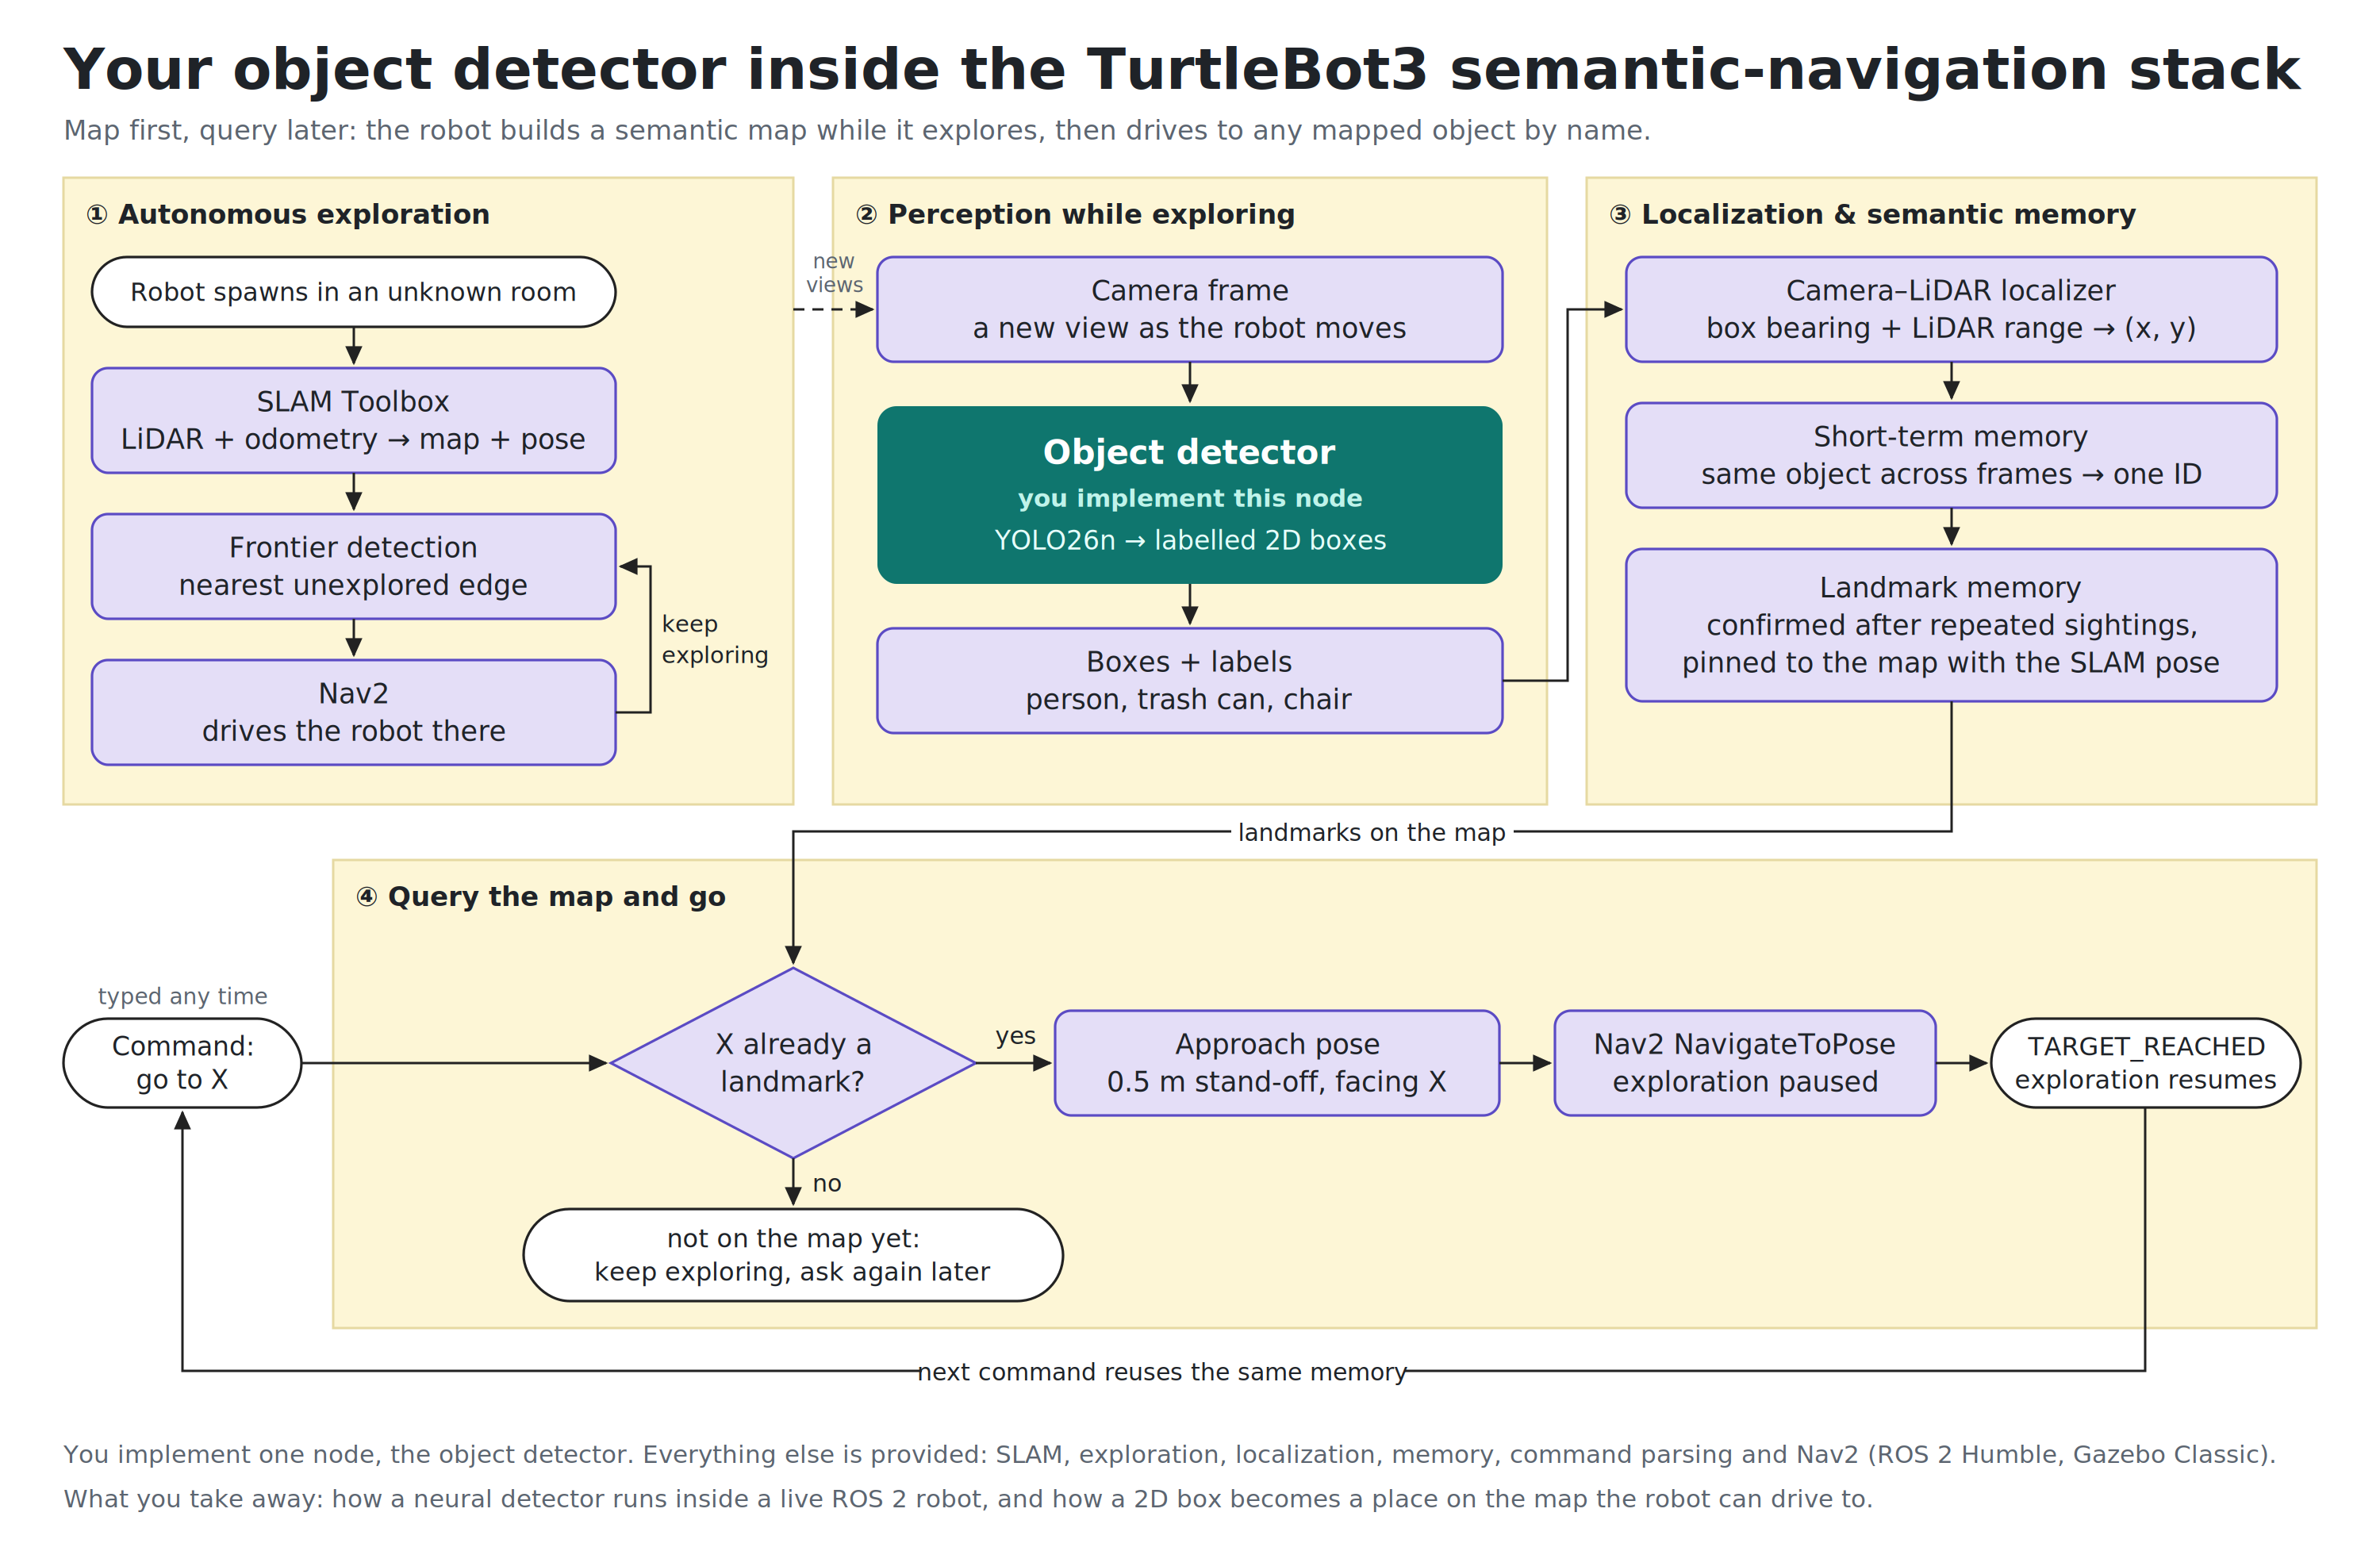
\includegraphics[width=\textwidth]{figures/system_overview.png}
\caption{The semantic-navigation stack. Figure taken from the course repository (\texttt{docs/media/system\_overview.png}). The object detector (dark box) is the part implemented in this lab.}
\label{fig:overview}
\end{figure}

\section{Giving and Parsing a Language Command}
\label{sec:command}

\textbf{Giving the command.} A command is a plain \texttt{std\_msgs/String} published on \texttt{/user\_command}, for example
\begin{verbatim}
ros2 topic pub --once /user_command std_msgs/String "data: 'go to the chair'"
\end{verbatim}
The coordinator node is the only subscriber. Its mode moves through
\begin{center}\small
\texttt{EXPLORING} $\rightarrow$ \texttt{SEMANTIC\_QUERYING} $\rightarrow$ \texttt{SEMANTIC\_NAV} $\rightarrow$ \texttt{TARGET\_REACHED} or \texttt{TARGET\_FAILED} $\rightarrow$ \texttt{EXPLORING}.
\end{center}
When a command arrives, the coordinator
\begin{enumerate}[leftmargin=1.5em]
\item cancels any goal it sent earlier,
\item publishes \texttt{false} on \texttt{/exploration\_enabled}, so the frontier explorer stops sending new goals,
\item switches to \texttt{SEMANTIC\_QUERYING}, and
\item forwards the text to the query node on \texttt{/semantic\_query\_node/command}.
\end{enumerate}
Its progress is printed on \texttt{/coordinator\_node/status}, one line per step.

\textbf{Parsing.} The query node parses the text with fixed rules (no language model). It lower-cases the text, replaces punctuation with spaces and splits forms such as \texttt{person3} into \texttt{person 3}. It first checks phrase aliases (\texttt{trash can}, \texttt{trashcan} and \texttt{bin} all mean \texttt{trash\_can}); these are matched as substrings, before any other word. Otherwise it takes the first word that names a known target. The known targets are the enabled entries of \path{semantic_targets.yaml}: \texttt{person}, \texttt{trash\_can} and \texttt{chair}. An integer right after the target (\texttt{person 2}, \texttt{person no. 2}) asks for one specific landmark.

\textbf{Selecting a landmark.} The query node only looks at the persistent landmarks published by the semantic map memory on \texttt{/semantic\_map\_memory\_node/landmark\_objects} (Section~\ref{sec:perception}). With an index it requires the exact id, for example \texttt{person\_2}. Without an index it picks the landmark with the smallest distance computed from its map coordinates. Because those coordinates are in the map frame, this is the landmark closest to the map origin, not to the robot. If no landmark of the class exists yet, the reply is \texttt{query failed: no active <name> in memory} and the robot goes back to exploring, so the robot cannot go to an object it has not mapped. On success the query node publishes a \texttt{SemanticQueryResult} message with the landmark id and its position in the \texttt{map} frame, and the coordinator moves to \texttt{SEMANTIC\_NAV}. Table~\ref{tab:parse} shows the result for the two example commands in the assignment and for the two commands in the demo video.

\begin{table}[H]
\centering
\footnotesize
\begin{tabular}{lll}
\toprule
Command text & Parsed target & Landmark selected \\
\midrule
\texttt{move to the person wearing green shirt} & \texttt{person}, no index & person closest to map origin \\
\texttt{go to the red chair} & \texttt{chair}, no index & chair closest to map origin \\
\texttt{move to the person in the white shirt} (video) & \texttt{person}, no index & person closest to map origin \\
\texttt{go to the black trash can} (video) & \texttt{trash\_can} (alias) & trash can closest to map origin \\
\texttt{go to person 2} & \texttt{person}, index 2 & exactly \texttt{person\_2} \\
\bottomrule
\end{tabular}
\caption{Parser and selection behaviour (\texttt{parse\_command} and \texttt{select\_target} in \texttt{src/tb3\_query/tb3\_query/query\_core.py}).}
\label{tab:parse}
\end{table}

Attributes such as colour are therefore not used. The parsed command keeps only the class and an optional index, and the detector reports classes only. In the provided worlds the person model wears a white T-shirt and the trash can is black, so in the video I described the objects as they look. The parser treats ``green shirt'' in exactly the same way: the words are skipped.

\section{From Camera Images to Objects on the Map}
\label{sec:perception}

\subsection{Object detector (my implementation)}

The Gazebo camera publishes $640\times480$ images on \texttt{/camera/image\_raw}. The provided \texttt{detector\_node} converts each image to a BGR array and calls \path{DetectorCore.infer()}.

\begin{itemize}[leftmargin=1.2em]
\item \textbf{\texttt{load()}} raises a \texttt{RuntimeError} if \texttt{ultralytics} cannot be imported and a \texttt{FileNotFoundError} if the weights file is missing, so that a broken setup fails at start-up with a readable message. Otherwise it loads the fine-tuned YOLO26n weights \texttt{tb3det\_yolo26n.pt}, whose three classes are \texttt{person}, \texttt{trash\_can} and \texttt{chair}, and moves the model to the configured device (CPU). It also logs a warning if the class whitelist names a label that the weights never output, because such detections would otherwise disappear without any message.
\item \textbf{\texttt{infer()}} raises an error if no model is loaded, runs \texttt{predict} with the confidence threshold 0.40 from \path{detector.yaml}, and returns one dictionary per box: the label exactly as the network names it (\texttt{result.names[int(box.cls)]}), the confidence as a float, the box as \texttt{[x1, y1, x2, y2]} in pixels of the original image (origin at the top-left corner, as ultralytics returns it), and \texttt{track\_id = None} because tracking is off. Boxes whose label is not in the whitelist are dropped. When nothing passes it returns an empty list.
\item \textbf{Optional thread cap.} If the environment variable \texttt{TB3\_DETECTOR\_THREADS} is set, \texttt{infer()} limits the number of CPU threads PyTorch uses. When it is not set, the detector behaves as before. Section~\ref{sec:results} explains why I needed it.
\end{itemize}

The node packs the list into a \path{vision_msgs/Detection2DArray} on \texttt{/detector\_node/detections} and draws the boxes on \texttt{/detector\_node/debug\_image}, which RViz shows (Figures~\ref{fig:dets} and~\ref{fig:views}).

In the self-test world of the instructions (Step 4), the detector reported exactly one \texttt{person} box (confidence 0.97), with about 20 detection messages per second.

\subsection{Localizer: box plus LiDAR gives a position}

The localizer turns the horizontal centre $u$ of a box into a bearing through the camera's horizontal field of view (HFOV $=62.2^\circ$, image width $W=640$):
\[
\theta = -\frac{u - W/2}{W/2}\cdot\frac{\mathrm{HFOV}}{2},
\]
so an object in the left half of the image has a positive bearing (to the robot's left, following the ROS convention). It then reads the latest LiDAR scan at that bearing, takes the median of the valid ranges in a window of $\pm 5$ rays (valid means between 1.0 and 3.3\,m), and converts the result to $x = r\cos\theta$, $y = r\sin\theta$ in the robot frame \texttt{base\_link}. Boxes whose centre lies within 40\,px of the left or right image edge are ignored, because a box cut off by the image border has a shifted centre and would point the LiDAR at whatever stands next to the object. This is also why the pixel convention in \texttt{infer()} matters: a wrong $x$ coordinate would make the LiDAR measure a different object.

\subsection{Short-term memory and the semantic map}

A short-term memory node, working in the robot frame, associates observations with the same label that fall within 1.0\,m of each other and smooths their positions. It republishes every object it has seen in the last 5\,s once per second. The semantic map memory transforms each of these observations into the \texttt{map} frame with the SLAM pose, snaps it to the nearest occupied blob of the occupancy grid (so that a landmark sits on something the LiDAR actually sees), and adds it to a candidate, which is an unconfirmed group of observations at one place. A candidate becomes a landmark after 8 such once-per-second observations for a person and 12 for a trash can or a chair. Landmarks receive ids such as \texttt{person\_0} and \texttt{person\_1}. When two labels are reported at the same place, the landmark keeps a count per label and is relabelled once another label has at least 1.5 times as many observations and has reached its own threshold. Landmarks appear in RViz as coloured spheres with their id (\texttt{/semantic\_memory\_markers}, Figure~\ref{fig:views}). Perception never pauses, so landmarks keep improving while the robot navigates.

\begin{figure}[H]
\centering
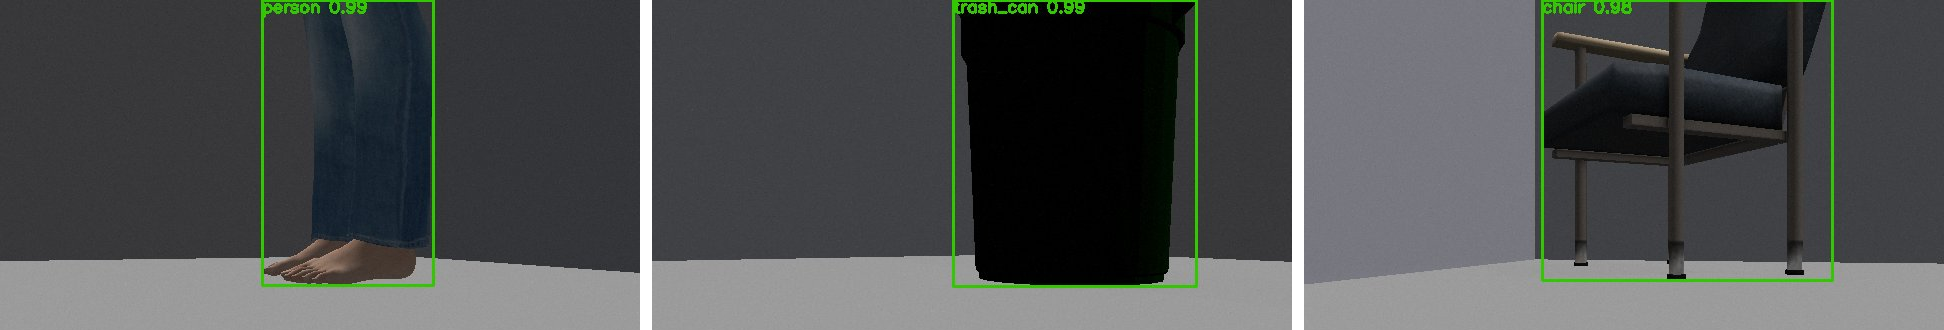
\includegraphics[width=\textwidth]{figures/detections.png}
\caption{Detector debug images recorded during my runs: \texttt{person} 0.99, \texttt{trash\_can} 0.99 and \texttt{chair} 0.98. The boxes and scores are the output of \texttt{infer()} drawn by \texttt{detector\_node} (top part of each $640\times480$ frame shown).}
\label{fig:dets}
\end{figure}

\begin{figure}[H]
\centering
\IfFileExists{figures/rviz_landmarks.png}{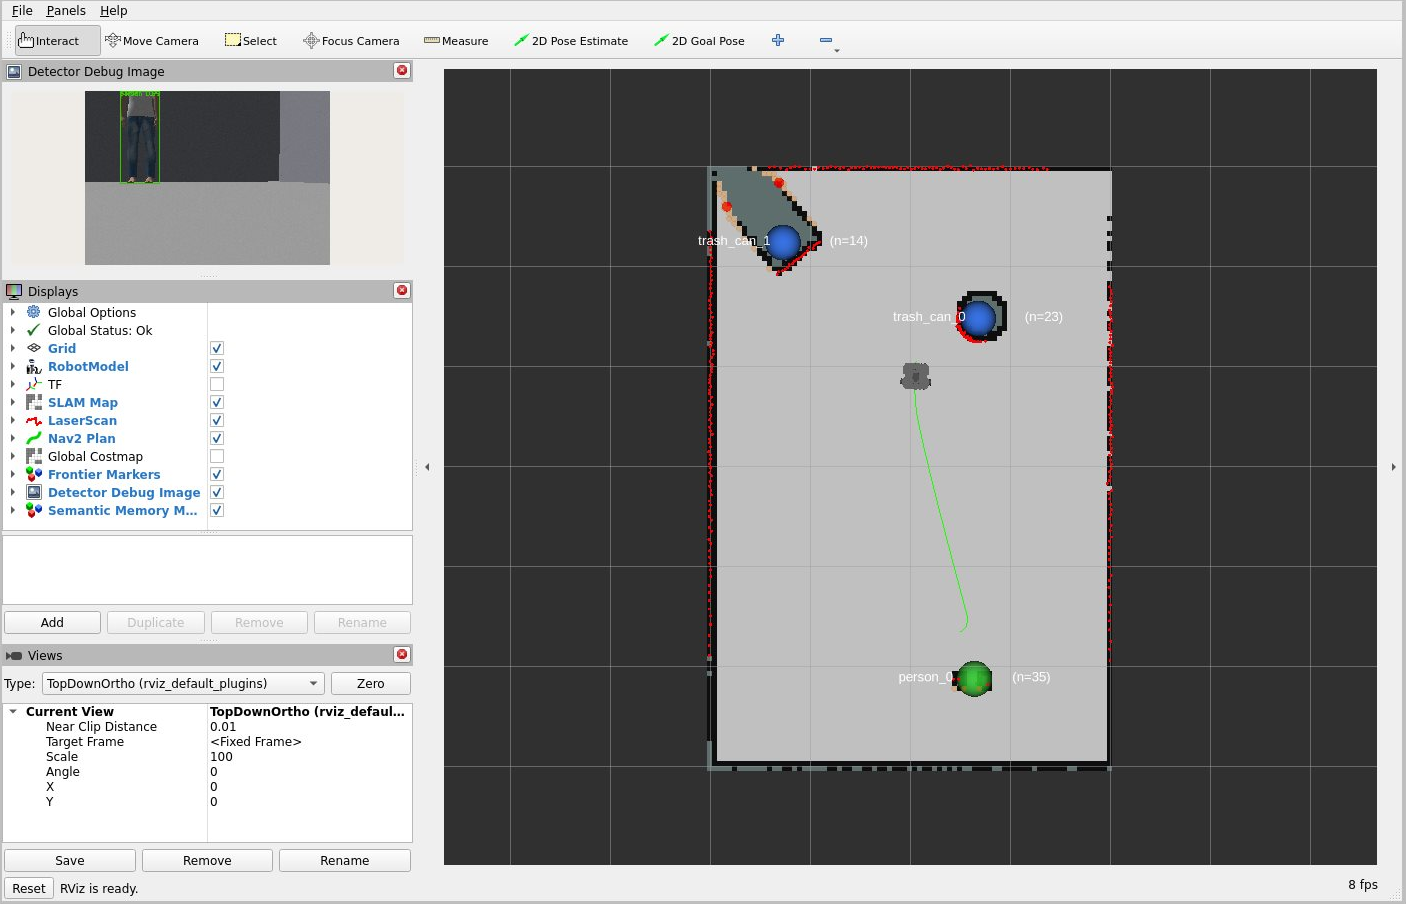
\includegraphics[width=0.82\textwidth]{figures/rviz_landmarks.png}}{\fbox{\parbox[c][5cm][c]{8cm}{\centering RViz screenshot}}}
\caption{RViz during the first command of the demo video (\texttt{move to the person in the white shirt}): the SLAM map, the laser scan (red), the Nav2 plan from the robot to the approach pose (green line) and the semantic landmarks (spheres with id and observation count). \texttt{trash\_can\_0} is the real trash can; \texttt{trash\_can\_1} sits on the chair (Section~\ref{sec:results}). The panel at the top left is the detector debug image.}
\label{fig:views}
\end{figure}

\section{The Constructed Map and Exploration}
\label{sec:map}

SLAM Toolbox, started in its synchronous online mode through \texttt{nav2\_bringup} with \texttt{slam:=True}, builds the occupancy grid \texttt{/map} from the LiDAR and the wheel odometry and publishes the \texttt{map}$\rightarrow$\texttt{odom} transform. The map is used in three places:
\begin{enumerate}[leftmargin=1.5em]
\item Nav2 plans on it through the global costmap.
\item The semantic map memory stores landmarks in its frame and snaps them to its occupied cells (Section~\ref{sec:perception}).
\item Frontier exploration uses it to decide where to look next.
\end{enumerate}

Exploration starts with a warm-up turn of $\pm45^\circ$. The frontier detector then marks free cells that touch unknown cells, groups them into clusters of at least three cells and keeps each cluster's centroid unless it lies in a high-cost area of the costmap. The goal assignment node sends the nearest acceptable centroid to Nav2, gives up on a goal after 20\,s and avoids failed goals for 90\,s. A command pauses exploration, and exploration restarts 3\,s after the command has finished.

\section{Driving to the Goal}
\label{sec:nav}

\textbf{Approach pose.} The nav adapter turns the landmark into an approach pose. Let $d$ be the landmark's distance from the map origin. The adapter places the goal $\min(0.5,\ d-0.3)$\,m in front of the landmark on the line from the map origin to the landmark, and turns the robot to face the landmark. The line starts at the map origin rather than at the robot because the target already arrives in the \texttt{map} frame; the course notes document this simplification (\path{NOTES.md}, Section~5.1). If $d<0.3$\,m the adapter publishes no goal at all, and the coordinator then waits in \texttt{SEMANTIC\_NAV} until the next command. For $d<0.8$\,m the goal lies less than 0.5\,m from the landmark, so the acceptance script skips such targets.

\textbf{Nav2.} The coordinator sends the pose to Nav2 as a \texttt{NavigateToPose} action and reports \texttt{Nav2 goal accepted -- robot is moving}. It cancels the goal itself if Nav2 has not finished after 60\,s. Nav2 runs with the stock Humble parameters (\path{nav2_bringup/params/nav2_params.yaml}). The NavFn planner computes a path on the global costmap. The DWB controller follows the path at 20\,Hz, using a local costmap built from the laser scan, and its velocity commands reach Gazebo's differential-drive plugin through \texttt{/cmd\_vel}. A goal checker accepts the goal within 0.25\,m and 0.25\,rad.

\textbf{After the goal.} When Nav2 reports success, the status becomes \texttt{[TARGET\_REACHED] Nav2 goal succeeded \ldots}; a Nav2 failure or the 60\,s timeout gives \texttt{TARGET\_FAILED}. In both cases exploration resumes after 3\,s, and the semantic map is kept for the next command.

Nav2 success only means that the robot reached the approach pose. The coordinator never checks the distance to the real object, so the course's acceptance test measures that distance against Gazebo ground truth and requires at most 1.2\,m. According to the course notes (\path{NOTES.md}, Section~6.1.1), the budget is the 0.5\,m stand-off, plus the bias of a landmark towards the robot (the LiDAR returns the near surface of the object, up to 0.36\,m for the chair), plus Nav2's goal tolerance of 0.25\,m, about 1.1\,m in total.

\section{Runs, Results and the Demo Video}
\label{sec:results}

\textbf{Setup.} Laptop with an Intel i9-12900H, 16\,GB of RAM and an RTX 3070 Ti Laptop GPU; Windows 11 with WSL~2 and Ubuntu 22.04. The detector runs on the CPU (PyTorch 2.5.1 CPU build, ultralytics 8.4.31). Following the repository's Windows page, I set \path{MESA_D3D12_DEFAULT_ADAPTER_NAME=NVIDIA} so that Gazebo renders on the discrete GPU; the default integrated GPU can make the simulated camera return empty frames. Gazebo ran at a real-time factor of 1.00.

\textbf{CPU load and the thread cap.} In my first runs \texttt{top} showed the detector process at about 850\% CPU. In ultralytics 8.4.31, \texttt{select\_device()} sets PyTorch to $\min(8, \mathrm{cores}-1)$ threads (\path{ultralytics/utils/torch_utils.py}). The WSL load average was 13 on 20 logical CPUs, and Nav2 reported \texttt{Control loop missed its desired rate}. I therefore added the optional thread cap of Section~\ref{sec:perception}. With 4 threads the detector used about 4 cores, and one frame took a median of 32.2\,ms instead of 44.7\,ms with 8 threads. Runs 4 and 5 in Table~\ref{tab:acc} and the demo video used \texttt{TB3\_DETECTOR\_THREADS=4}.

\textbf{Acceptance runs.} \texttt{scripts/acceptance\_run.sh} starts the five launch terminals of the README (T1--T5), waits until the expected landmarks exist (at most 600\,s), sends the commands and scores the robot's final position against Gazebo ground truth. I ran it \NRuns{} times, and Table~\ref{tab:acc} lists every run in order. The detector commits differ only in the whitelist warning and the thread cap; the detections they produce are the same.

\begin{table}[H]
\centering
\small
\begin{tabular}{llrrrl}
\toprule
Command & Landmark & Landmark error (m) & Final distance (m) & Time (s) & Result \\
\midrule
\AcceptanceRows
\bottomrule
\end{tabular}
\caption{All acceptance runs, in the order I ran them (\texttt{report/results/*.json}). Landmark error is the distance between the selected landmark and the real object. Final distance is between the robot and the real object after the command; the pass mark is 1.2\,m. The italic line under each run summarizes what the logs showed. $^{*}$The landmark is the person standing on the map origin; the nav adapter cannot build a goal there (Section~\ref{sec:nav}), so the script skips it.}
\label{tab:acc}
\end{table}

\textbf{What the runs show.} Every landmark that a command selected was close to the right object: the \NLandmarks{} selected landmarks were \LmErrMin--\LmErrMax\,m from the real objects. Navigation reached the target for \NReached{} of the \NNavigable{} commands that had a landmark, and every reached target ended \DistMin--\DistMax\,m from the object, inside the 1.2\,m mark. No run completed all three commands of the three-target world. The failures have the causes below. One of them is a perception problem (the chair), which comes from the provided weights; none of them traces back to a bug I found in \texttt{infer()}.

\textbf{Demo video.} The video uses the trash can instead of the chair, because in that run the chair was labelled as a trash can (\texttt{trash\_can\_1} in Figure~\ref{fig:views}). The video (\path{videos/lab3a_demo.mp4}, 56\,s) was recorded in the three-target world with the final detector. The left side is the RViz window, the top right is the detector debug image, and the caption shows each command exactly as it was published and what the parser makes of it. The robot explored for 215\,s before the person and trash-can landmarks existed; this part is shown at six times real speed. The first command, \texttt{move to the person in the white shirt}, was reduced to the target \texttt{person}, and the robot reached \texttt{person\_0} after 18.3\,s. The second command, \texttt{go to the black trash can}, was reduced to \texttt{trash\_can}, and the robot reached \texttt{trash\_can\_0} after 11.6\,s. Both commands are shown at twice real speed. In this world the real trash can is closer to the map origin than the chair, so the query node chose the real trash can.

\begin{itemize}[leftmargin=1.2em]
\item \textbf{SLAM stopped (runs 1 and 4).} The \texttt{map}$\rightarrow$\texttt{odom} transform stopped updating partway through the run. SLAM Toolbox logged no error; it simply stopped publishing the transform. Nav2 then logged \texttt{Transform data too old when converting from map to odom} and aborted goals even when the robot was already close (in run 4 the robot ended 0.31\,m from the person, but the goal was aborted). During run 1 I was installing a package in the same WSL instance, but run 4 had nothing else running and the thread cap set, so the cap did not remove this problem.
\item \textbf{Chair seen as a trash can (runs 1 and 4).} A \texttt{trash\_can} landmark formed at the chair, no \texttt{chair} landmark appeared within 600\,s, and \texttt{go to chair} returned \texttt{no active chair in memory}. Only in run 3 was the chair mapped as a chair (landmark 0.27\,m from it).
\item \textbf{Controller timeout (run 3).} The robot did not reach the chair. The controller server logged \texttt{Controller patience exceeded}, meaning DWB found no valid velocity command for too long, and the coordinator cancelled the goal at its 60\,s timeout.
\item \textbf{Observations at the wrong object.} The semantic map memory counts every label that arrives at a landmark. In one run the person landmark had also collected 12 \texttt{chair} and 11 \texttt{trash\_can} observations, and in most of my runs of the three-target world a \texttt{trash\_can} landmark formed at the chair. I have two possible explanations, neither of them tested. The localizer pairs each detection with the latest laser scan without time synchronization, and the short-term memory republishes robot-frame positions for up to 5\,s, which the map memory transforms with the current pose. In both cases, an observation made before the robot turned can end up on another object.
\item \textbf{Person on the map origin.} In the five-person world one figure stands on the map origin. Whatever id this figure receives (\texttt{person\_0} in run 2, \texttt{person\_1} in run 5), the command for that id cannot be served (Section~\ref{sec:nav}). Plain \texttt{go to the person} picks the person closest to the map origin, which is also this figure, so it stalls in the same way. This is a limitation of the provided nav adapter.
\end{itemize}

\section*{AI Use Statement}

I used Claude (Anthropic) through Claude Code as an assistant in this lab. It installed ROS~2 and the course workspace in WSL, implemented and unit-tested \texttt{load()} and \texttt{infer()} following the instructor's outline, ran the acceptance runs, recorded the demo video, and drafted this report. I directed the work and reviewed the code, the results and the report.

\end{document}
